\documentclass[a4paper,oneside]{article}

  \usepackage{graphicx}
  \usepackage{subcaption}
  \usepackage{xcolor}
  \usepackage{hyperref}
  \usepackage[cm]{fullpage}
  \usepackage{booktabs}
  \usepackage{lmodern} 
  \usepackage[T1]{fontenc}
  \usepackage{amsmath}

\begin{document}
  \section*{The hypothetical adaptive value of the generalized growth arrest and the constraints for a successful sex event}
    Molecular, biophysical and chemical data discussed above unequivocally show that \textit{P.~multistriata}, during events of mating and gametogenesis, blocks growth and mitosis for a few days --- three in the experiment discussed here, and up to six in the one discussed by Scalco et al. (2014).
    Also, cell number decreases, very likely for enhanced mortality due to the gametogenesis.

    To analyze the impact of such behaviour on population dynamics, we developed a simple process-based model of growth dynamics during the sexual reproduction event, where net growth is the balance between size-dependent cell growth and death.
    The model is conceptually zero-dimensional, and the initial conditions consider the minimal cell concentration recorded by Scalco et al. (2014) as gametogenesis trigger.

    {\color{red}\textbf{Nota 1 Marina
    {\color{blue}[threshold cell concentration, ovvero 4,000 cells/ml per ciascun parental strain? che roughly corrisponde alla ca 10,000 cell per entrambi i parentali E' un dettaglio, scusa]}:
    %
    la concentrazione iniziale {\`e} di 4000 cellule in totale. Il modello non distingue tra mating types ma l'assunzione implicita {\`e} che siano 2000+2000 che {\`e} poco pi{\`u} grande del minimo riportato nel paper di Ele a p. 820 inizio seconda colonna ed in fig 3a}
    }

    Cell numbers and available Nitrogen are expressed as abundance and concentration, respectively.
    \
    The simulation starts with a cell population ($P$) that enters the sexual reproduction phase after reaching a threshold value of a few thousand cells per ml (see Scalco et al., 2014).

    During this phase of variable length, the population stop growing and experience a prolonged burst of extra mortality.

    {\color{red}\textbf{Nota 2 Marina
    {\color{blue}[la mortalit{\`a} pare confinata ai primi due giorni direi, sia nei due exp di Scalco (turbolenza e still condition che in quello di Rossella). Interpreto come mortalit{\`a} valori negativi di growth rate: OK?]}:
    %
    Attualmente ci sono due parametri che variano. $t_{F_1 I}$ e $t_{A E}$. $t_{A E}$ {\`e} il giorno in cui finisce l'arresto della crescita e nelle simulazioni varia da 2 a 6 giorni (v.\ tabella 1). L'extra mortalit{\`a} per gametogenesi dura 1 giorno in meno di $t_{A E}$ e quindi dipende da $t_{A E}$ (v.\ relazioni con le parentesi graffe). Il valore di $t_{A E}$ tiene conto degli exp.\ di Rossella e di quelli di Ele le cui figure suggeriscono che un $t_{A E}$ di 6 giorni sia realistico menre vincolare l'extra mortalit{\`a} alla fase di GA ci {\`e} sembrato logico perch{\`e} le due risposte dovrebbero essere collegate. Comunque si tratta di un'esplorazione e serve per vedere che succede cambiando la durata del GA e la durata dell'extra moratlit{\`a} potrebbe essere fissata a 2 giorni se pensiamo sia preferibile. $t_{F_1 I}$ {\`e} invece il giorno in cui nascono le prime figlie ed attualmente {\`e} posto a 3 (v.\ tabella 1)}
    }

    Within the same span, a $P$ fraction will undergo gametogenesis and generate an offspring population ($F_{1}$) that will start to grow the moment ($t_{F_{1}I}$) it appears.
    After $t_{AE}$ days, the growth arrest will end and $P$ will resumes its growth alongside $F_{1}$.

    {\color{red}\textbf{Nota 3 Marina
    {\color{blue}[quando possiamo dire che che la growth arrest termina? Dopo i primi due giorni in cui {\`e} negativa, la growth rate diventa positiva, ma {\`e} sempre pi{\`u} bassa rispetto alla growth rate dei parentali in mono-coltura. Per questo suggerivo di calcolare la growth rate in ogni singolo giorno]}:
    % 
    Come detto sopra la durata del GA varia da 2 a 6 giorni (nella figura 2 ogni panel rappresenta l'effetto di una specifica durata) e questo vincola anche il numero di giorni di extra-mortalit{\`a} per l'extra mortalit{\`a}. I tassi di crescita variano solo in relazione alla taglia (v.\ le equazioni a pag. 1 ricavate a suo tempo da Domenico e la fig.1b) e per le parentali, che sono piccole, le variazioni nei giorni in cui ricominciano a crescere sono trascurabili. I tassi di crescita sono comunque quelli delle cross e non quelli delle parentali isolate.}
    }

    During the entire course of the simulation (set to ten days) cell growth is modulated by competition over Nitrogen and by cell size via an allometric relationship (see D'Alelio et al., 2010).

    {\color{red}\textbf{Nota 4 Marina
    {\color{blue}[ma l'azoto non {\`e} limitante nei nostri esperimenti. Voi assumete che lo possa essere alla Kolmogorov scale, o boundary layer o qualcosa del genere, ovvero la scala dell'ambiente attorno alla cellula/e? Questo {\`e} un punto che non mi {\`e} chiaro e che dovrebbe essere menzionato/definito. Mi sbaglio?]}:
    %
    I tassi di crescita utilizzati sono quelli osservati in laboratorio in condizioni di disponibilit{\`a} in eccesso di azoto, tuttavia sono sostanzialmente coerenti con quelli inferiti dalla crescita in situ derivata dalla riduzione di taglia osservata in situ, per{\`o} su intervalli temporali pi{\`u} lunghi (di fatto interpolando su settimane). Poich{\'e} per duplicarsi le cellule devono assimilare azoto l'assunzione che facciamo {\`e} che in natura la comunit{\`a} sia intorno allo stato stazionario, cio{\`e} non ci sia azoto inorganico disponibile se non quello derivato dal riciclo. Questo corrisponde bene con l'analisi che facemmo col lavoro di Domenico, cio{\`e} che la fase di riproduzione di \textit{Pm} coincideva con diverse concentrazioni di clorofilla totale, quindi diversi livelli di capacit{\`a} portante del sistema ma non a condizioni di significative quantit{\`a} di nutrienti inutilizzati. Il GA mette a disposizione l'azoto che verrebbe utilizzato dalle parentali qualunque sia l'origine. Questo potrebbe essere utilizzato da tutti i componenti della comunit{\`a}. La precisazione che facciamo {\`e} che l'azoto che avrebbero usato le parentali, che se non avessero avviato la fase riproduttiva, avrebbero piu' o mantenuto i livelli di abbondanza precedenti, venga usato totalmente dalle cellule figlie, perch{\`e} ipotizziamo che le cellule figlie restino molto vicine alle parentali e che quindi l'azoto che avrebbero utilizzato loro possa essere utilizzato dalle figlie. L'assunzione aggiuntiva {\`e}, un p{\`o} pi{\`u} forte, e forse discutibile, {\`e} che il tempo di riciclo dell'azoto sia rapidissimo per cui anche il contenuto di azoto delle parentali morte sia subito disponibile per le figlie. Lo scenario {\`e} plausibile se il tempo di dispersione delle cellule, parentali e figlie {\`e} pi{\`u} lento del tempo della diffusione chimica, che {\`e} quella che porta l'azoto mentre la perdita di azoto per diffusione chimica {\`e} neutralizzato dall'assimilazione delle figlie. Tutto questo implica che ci siano porcessi di micropatching di molte cellule che si dividono i ruoli (v.\ sotto)}
    }

    {\color{red}\textbf{Nota 5 Marina
    {\color{blue}[quindi avete definito che le cellule parentali hanno taglia diversa? questo era in caso nell'exp di Eleonora perch{\'e} volevamo distinguere i MT in quanto sembrava a quei tempi che uno dei MT si bloccasse pi{\`u} dell'altro. Cambiano molto le cose se i parentali hanno taglie diverse? ovvero 1.\ la pi{\`u} piccola e la pi{\`u} grande nell'ambito della taglia per il sesso o 2 entrambi grandi o 3 (entrambi piccoli). Magari anche questi sono dettagli insignificanti x il modello\dots]}:
    %
    Nel modello le taglie dei mating type {\`e} la stessa non si considerano le differenze del setup sperimentale e il tasso di crescita utilizzato e ricavato dall'exp {\`e} probabilmente quello medio tra le due taglie. Mettere taglie diverse cambierebbe nella disponibilit{\`a} di azoto e quindi della abbondanze finali, ma non nella descrizione del processo.}
    }

    A fundamental assumption, discussed later in the text, is that parental and daughters cells share a common, exclusive space, so that only $P$ and $F_{1}$ compete for N made available in such space.

    {\color{red}\textbf{Nota 6 Marina
    {\color{blue}[da questo io capirei che l'arresto della crescita {\`e} determinato da un fattore esogeno, ovvero il raggiungimento della carrying capacity: quando hanno assimilato tutto l'azoto si fermano]}:
    %
    La crescita delle cellule dipende dal massimo tasso di crescita intrinseco dipendente dalla taglia (il $\lambda$ nelle equazione) e dalla disponibilt{\`a} di azoto (il termine $\kappa$ nelle equazioni 1 e 2) quindi quando l'azoto che era potenzialmente disponibile o contenuto nelle parentali finisce si fremano. In realt{\`a} noi ci fermiamo dopo dieci giorni di simulazione. Quello che succede dopo {\`e} quello che succede a tutta la comunit{\`a} cio{\`e} {\`e} un nuovo steady state, con le figlie presenti.}
    }

    This assumption is translated in the model as a decrease in growth rate as the total population ($F_{1} + P$) converges toward the carrying capacity, set as the total nitrogen content of initial parental cells.
    
    To understand better how event timing and response amplitudes impact over $F_{1}$ recruitment success, we compared simulation outputs across selected parameters range.
    Our selected parameters are the $P$ fraction that will generate $F_{1}$ ($\alpha$), gametogenesis-induced extra mortality of parental cells ($d$), duration of the growth arrest ($t_{AE}$), and growth rates ratio among parental and initial cells ($r_{P}:r_{F_{1}}$)

    {\color{red}\textbf{Nota 7 Marina
    {\color{blue}[il numero delle F1 include sia le F1 che `originano' da un evento di sesso che le F1 che si duplicano. Questa alpha sarebbe l'efficienza della riproduzione sessuata direi, ovvero la frazione di eventi sessuati che sono andati a buon fine? potrebbe forse essere stimato considerando il numero delle auxospore considerando che l'auxospora che vedi il giorno $x$ si sia trasformata in F1 al giorno $x+1$? Nei filmati che facevo vedere l'altro giorno, Eleonora aveva stimato che le auxospore ci mettono ca 10--15 ore a svilupparsi. Questa potrebbe essere una stima del successo della ripr sessuata? Quando i due strain si incontrano vengono prodotti molti gameti/zigoti (v dati di rossella, parecchie centinaia) ma molti muoiono perch{\`e} non si accoppiano. Si formano molte meno auxospore che rappresentano le coniugazioni che vanno a buon fine. Le auxospore permangono a lungo nell'exp di Rossella.]}
    %
    Questa {\`e} un'incertezza non risolvibile con le osservazioni perch{\'e} non si riesocno a distingure le $F_1$ dalle loro figlie. Per{\`o}, data la taglia le $F_1$ ci mettono lameno due giorni a riprodursi quindi l'errore dovrebbe essere relativamente piccolo tra i dati che usiamo e le assunzione del modello}
    }

    We deployed an interactive version of the model at the URL \url{https://arfalas.shinyapps.io/pns_toy/}, code and figures are available on \url{https://github.com/bhym/Stec} ({\color{red} currently private})
%
  \section*{Model description}
    Parental ($P$) and offspring ($F_{1}$) dynamics are defined as ODE:\@
    %
    \begin{align}
      \frac{dP}{dt}     &= \kappa \mu_{P} P - \delta P \\
      \frac{dF_{1}}{dt} &= \kappa \mu_{F_{1}} F_{1}
    \end{align}
    %
    where $\kappa$ is the competition for N, defined as
    \[
      1 - \frac{{[N]}_{t}}{1.2{[N]}_{t=0}}
    \]
    with 
    \[
      [N_{t}] = {[P]}_{t} {[N]}_{P} + {[F_{1}]}_{t} {[N]}_{F_{1}}
    \]

    $\mu_{P}$ and $\mu_{F_{1}}$ are defined as
    \[
      \mu_{P} =
        \begin{cases}
          0                    & \mbox{if } t <    t_{AE} \\
          \lambda_{P}(t) r_{P} & \mbox{if } t \geq t_{AE}
        \end{cases}
      \qquad;\qquad
      \mu_{F_{1}} = 
        \begin{cases}
          0                            & \mbox{if } t <    t_{F_{1}I} \\
          \lambda_{F_{1}}(t) r_{F_{1}} & \mbox{if } t \geq t_{F_{1}I}
        \end{cases}
    \]
    with $\lambda_i(t)$ representing allometric scaling on length ($L$), defined as
    \[
      \lambda_{i}(t) = 0.25 + 0.04 L_{i}(t) - 0.0005 L_{i}{(t)}^{2}
    \]
    Length dynamics are based on cell's age ($a$) and are defined by the rule
    \[
      L_{i}(t) = L_{0,i} - 0.1 a(t) \hspace{8mm}\text{with $i$ either $P$ or $F_{1}$}
    \]
    Age is counted from the appearance of the population, and does not increase during GA.\@

    Finally, $\delta$ is an extra mortality term defined as
    \[
      \begin{cases}
        d & \mbox{if } t < t_{AE} \\
        0 & \mbox{if } t > t_{AE}
      \end{cases}
    \]
    The parameters values and ranges are reported in \textbf{Table~\ref{tbl1}}.
    %
    \begin{table}
      \centering
      {%
        \begin{tabular}{@{}llccr@{}}
          \toprule
          \textbf{Variable}&\textbf{Meaning} & \textbf{Units} & \textbf{Value} & \textbf{Reference}\\
          \midrule
          ${P}_{0}$       & initial concentration of $P$ cells         & cells/ml          & 4E3         & Experiment detailed in the paper\\
          $\alpha$        & fraction of $P$ that will generate $F_{1}$ & ---               & [0.01, 0.2] & Explored via simulations\\
          $r_{P}$         & net growth rate of $P$                     & $\text{day}^{-1}$ & [1, 3]      & Explored via simulations\\ 
          $r_{F_{1}}$     & net growth rate of $F_{1}$                 & $\text{day}^{-1}$ & 1           & ---\\
          $t_{AE}$        & end day of the growth arrest               & day               & [2,6]       & Explored via simulations\\
          $t_{F_{1}I}$    & day of appearence of the offspring         & day               & 3           & Experiment detailed in the paper\\
          $L_{0,P}$       & starting length for $P$ cells              & $\mu$m            & 40          & Experiment detailed in the paper\\
          $L_{0,{F_{1}}}$ & starting length for $F_{1}$ cells          & $\mu$m            & 80          & Experiment detailed in the paper\\
          $d$             & gametogenesis-induced extra mortality      & day               & [0.1, 0.9]  & Explored via simulations\\
          \bottomrule
        \end{tabular}
       }
      \caption{Values and ranges for model parameters}\label{tbl1}
    \end{table}
%
  \section*{Results and Discussion of the simulations}
    \textbf{Fig.~\ref{fdyn}} shows the relative variation of allometric growth (\textbf{plot {\color{blue}\textit{a}}}) as derived from the equation reported above.
    Considering the time interval chosen for the simulation (ten days), the size reduction of $P$ and $F_{1}$ (\textbf{plot {\color{blue}\textit{b}}}) is negligible and, with it, the change in the growth rate of $P$ and $F_{1}$, with a significantly slower growth rate for $F_{1}$ due to their larger size.
    \textbf{Plots {\color{blue}\textit{c}}} and {\textbf{\color{blue}{\textit{d}}}} show the variation in abundance of $P$ and $F_{1}$ for two different sets of parameters used for the simulation.
    These plots provide a demonstration of the dynamics that the model simulates.
    A slower growth rate of $P$ ($r_p=1$, \textbf{plot {\color{blue}\textit{d}}} vs $r_p=1.82$, \textbf{plot {\color{blue}\textit{c}}}) that leaves more nitrogen available favours the growth of $F_{1}$, thus producing a greater abundance of $F_{1}$ and a lower abundance of $P$.

    The ten days length for growth arrest was chosen arbitrarily as a realistic time interval during which parental and daughter cells could remain close one to the other in a low sheared flow regime, so that the hypothesis of resources sharing could hold.
    The time spent in close vicinity by cells in a viscous regime  --- as the one we found in situ --- has been seldom analyzed in detail (see Jenkinson \& Wyatt, 1992 [Journal of Plankton Research, 14:1697--1721]).
    However, we assume that to permit mating, which implies direct contact among mates, several cells should converge by some mechanism --- for example, the one hypothesized by Botte et al., 2013 [J. Plankton Research 35: 914--918] and recently supported with observations by Font-Mu{\~n}oz et al.~(2019) [PNAS 116:15997--16002].
    On the basis of this assumtpion, our scenario would simulate local aggregations of cells, whose reproduction is favoured by the reaching of what we define threshold density.
    This concentration should be enough to trigger gametogenesis by chemical signal exchange ({\color{green}\textbf{ref}}).
    Once the gametogenesis starts all the involved cells stop growing and some individuals will form gametes, likely because the triggering caugth them in a specific phase of the cell cycle.
    Only a part of these gametes will encounter the opposite mating type, and only some of these will successfully complete the other phases,producing an $F_{1}$ generation (e.g., Scalco et al.~2014).
    Eventually, those unable to mate or complete gametogenesis will die.
    These considerations are compatible with the observed negative growth rate of $P$, and are formulated in the model as extra mortality ($d$).

    Assuming that auxospore formation scales with the encounter rate among mates, the number of auxospore formation should positively covary with the number of cell deaths due to unsuccessful encounters.
    This covariation would favour the $F_{1}$ growth, thus favouring better recruitment.
    In the following we discuss the main patterns resulting from simulations where the different parameters were varied, in all possible combinations, within the ranges reported in \textbf{Tab.}~\ref{tbl1}
    As the main output variable, we focused on the recruitment success of the offsprings --- quantified as the ratio between $F_{1}$ and $P$ ($r_p : r_{F_{1}}$) --- after ten days from the start of mating.

    Top row in \textbf{Fig.}~\ref{swep} show the ratio between the abundance of $F_{1}$ and that of $P$ after ten days of simulation for the growth rates ratio of $F_{1}$ and $P$ ($r_P : r_{F_{1}}$ on the $Y$ axis) vs $d$, the extra mortality ($X$ axis).
    The colours correspond to different ranges in the values of the decimal logarithm for the abundance ratio, e.g., $\log_{10}(F_{1}/P)$ and each plot displays the result for different durations of the growth arrest ($t_{AE}$).
    While $F_{1}$ will always be lower than $P$ (values of $\log_{10}(F_{1}/P)$ always lower than $0$), if the arrest persist more than four days a positive feedback appears between  abundance ratio and both net growth rates ($r_P : r_{F_{1}}$) and extra mortality $d$.
    In the more favourable scenarios, the ratio in abundance among $F_{1}$ and $P$ would be larger than $0.17$ (6 days of GA, dark green areas on the lower left).
    The lower row of the same figure shows the log-ratio among $F_{1}$ and $P$ abundances for various growth rate ration ($r_P : r_{F_{1}}$ on the $Y$ axis) vs the fraction of parental cells that generated daughter cells $F_{1}$ ($\alpha$), through auxospore formation.
    Success in recruitment appears to increase $F_{1}$ success, while growth rate ratio seems to affect it only for longer duration of growth arrest.

    We report the values of $\log_{10}(F_{1}/P)$ for different combinations of the parameters as supplementary tables \textbf{Table~\ref{tbl2}}..
    Overall the simulation provides a quantitative assessment of the number of $F_{1}$ that accumulate after ten day from the start of gametogenesis in relation to the number of mating cells and show that:
    1.\ only in extreme scenarios $F_{1}$ abundance will be equal or higher than $P$ and
    2.\ that the biological constrains of gametogenesis (growth arrest and extra death) due to resetting of cell physiology are compensated by an advantage for the $F_{1}$, mimicking a sort of maternal care.

    The constraints imposed by the series of events leading to \textit{Pm} recruitment also suggest that blooming is advantageous because increase the number of initial cells, thus allowing for a better seeding of the community with the new generation.
    Furtmermore, the concentration increase during bloom has a strong positive feedback on mating --- itself scaling with parental cell abundance, related to $\alpha$ in the model --- because it boost encounter rate.
    D'Alelio et al. (2010) inferred form data and modeling that the life cycle of \textit{Pm} consists of two phases characterised by opposite growth rate trends (slow vs fast).
    The shift in rates is collective and appears during bloom events, during which cells prepare for sexual reproduction.
    Identifying the triggers of this collective process would shed light on the long lasting debate on the relative weight of proximate vs ultimate factors (10.1126/science.1210879) and on the main drivers of the population dynamics of several diatoms.

    Relaxing the assumption that all the nitrogen left unused by blocked parental cells or regenerated from their death is used by the daughters with the possibility that part of it would go to other species in the community would just decrease the recruitment success but would produce an advantage for the other species in the community.
    In SM, we report the impact on the structure of the community and species succession of a sexual reproduction event in a simulation with a biogeochemical model reproducing the conditions of a North Atlantic site.
    Diatom sex events may be one of the factors that affect phytoplankton succession and changes in community structure in nature.
    %
    \begin{figure}[p]
      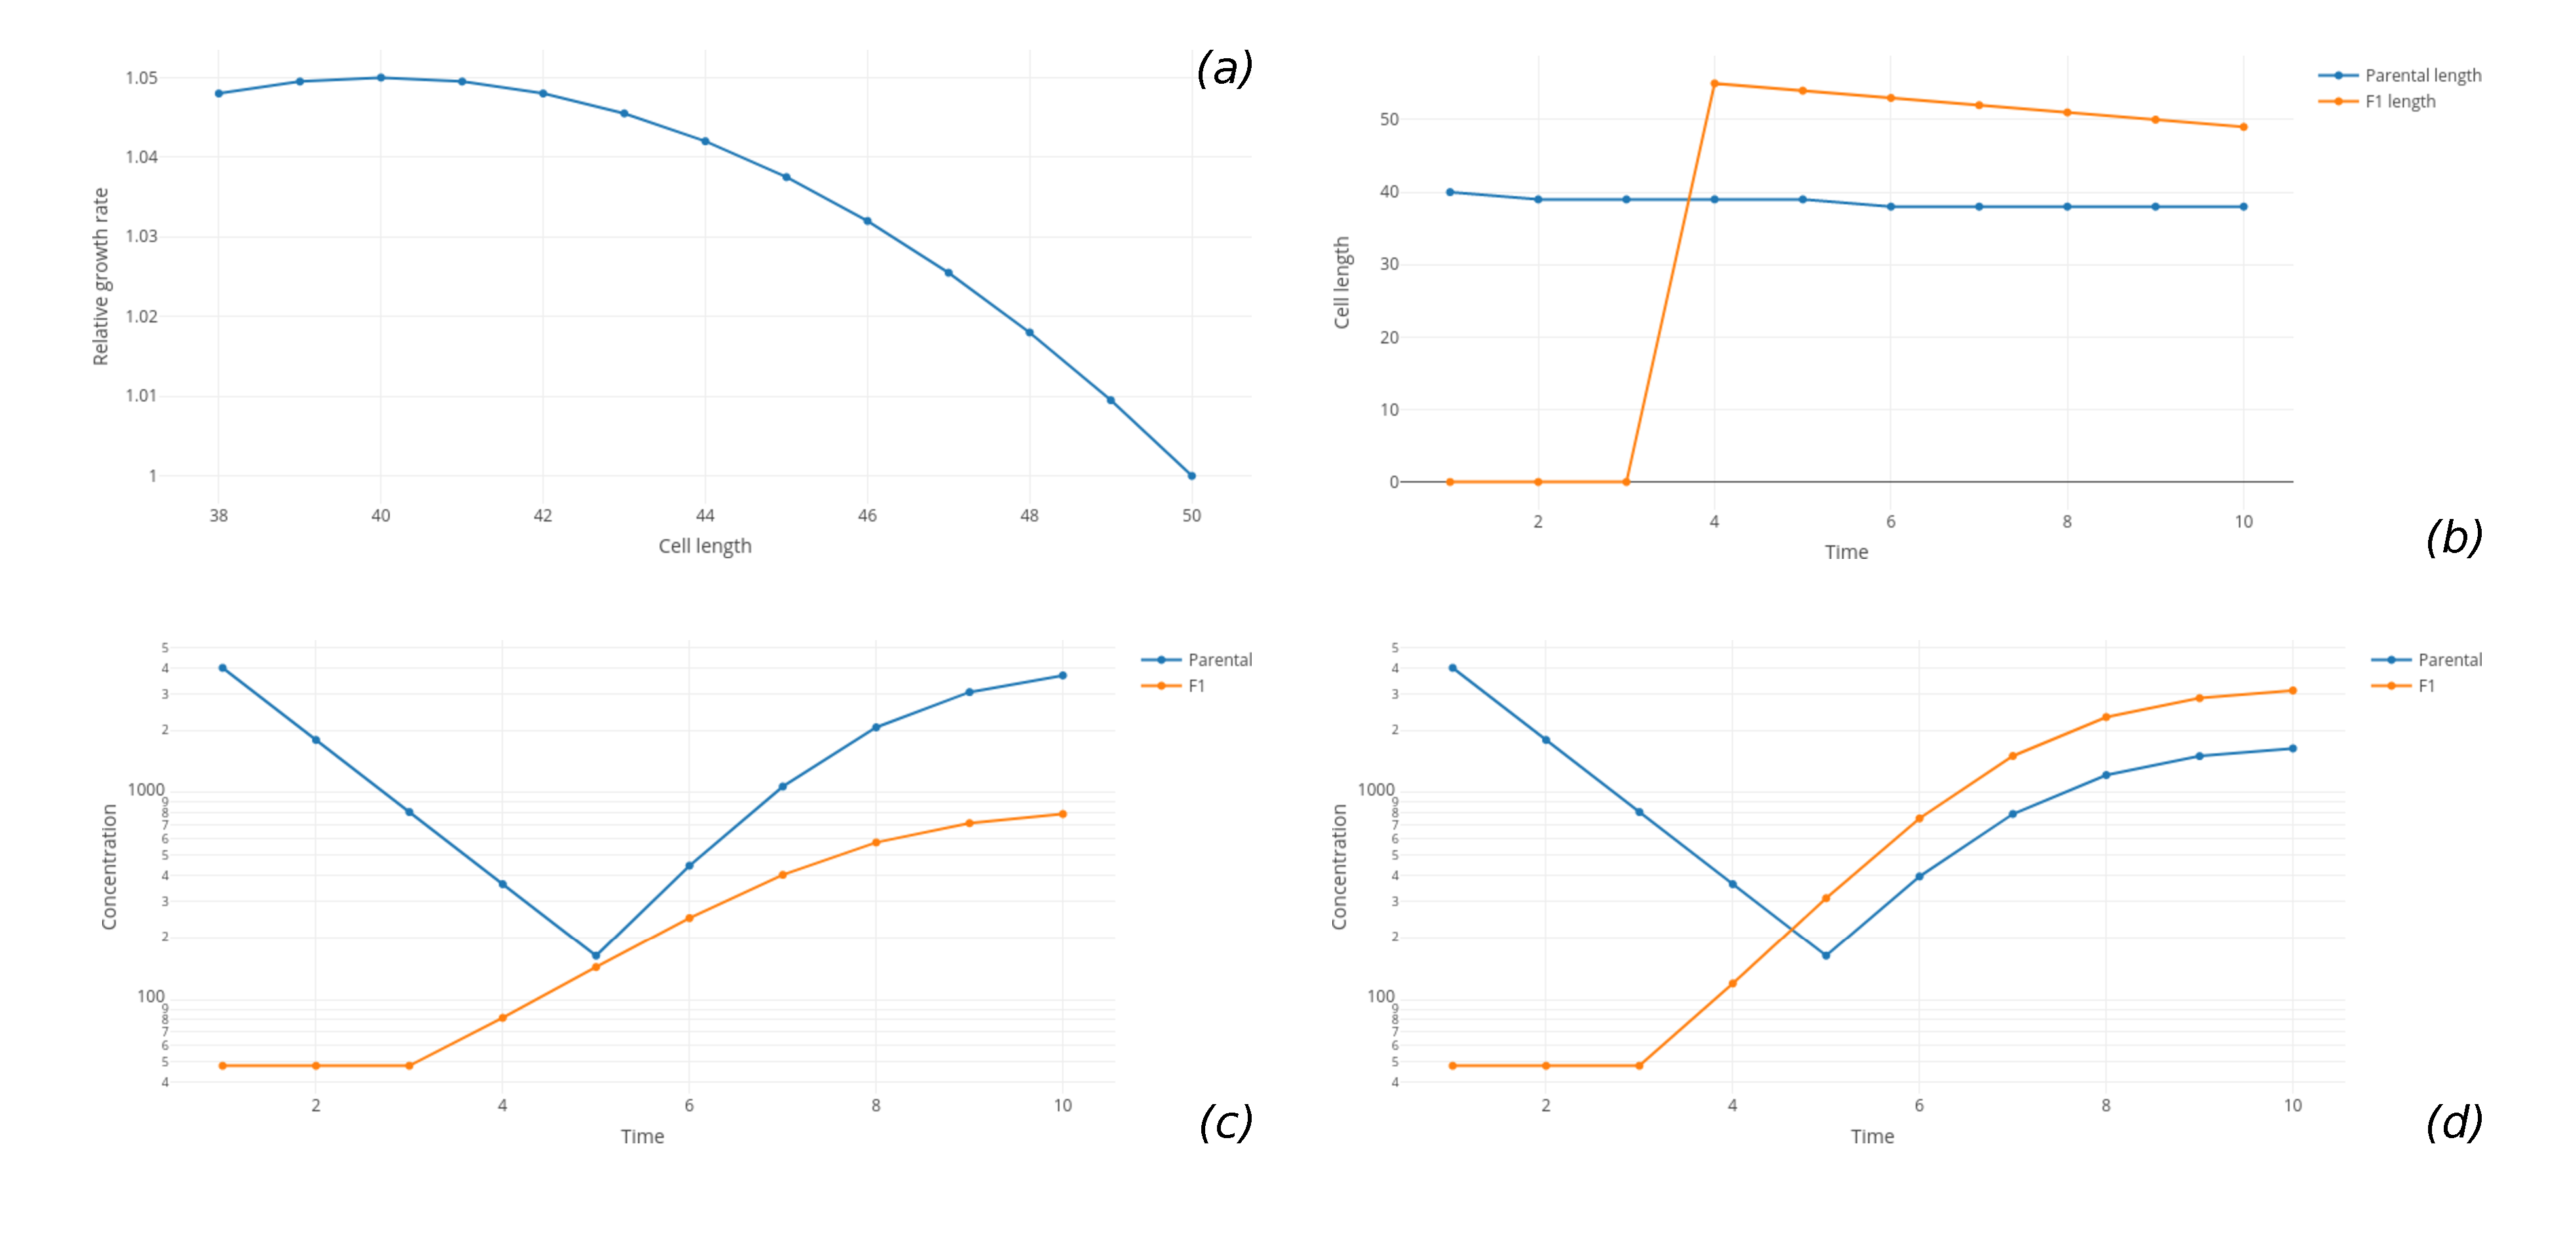
\includegraphics[width=\linewidth]{imgs/Figpan.pdf}
      \caption{\textbf{Simulated size dependent growth and impact on the population dynamics} ---
        {\color{blue}\textit{(a)}} dependence of specific growth rate on cell length;
        {\color{blue}\textit{(b)}} Size reduction for the two sub-populations;
        examples of simulation outputs whith $r_{p} >r_{f1}$ (1.06 and 0.58, respectively) {\color{blue}\textit{(c)}} and $r_{p} = r_{f1}$ {\color{blue}\textit{(d)}}.
        In {\color{blue}\textit{(c)}} and {\color{blue}\textit{(d)}}: $\alpha=0.012, d = 0.8$, all the other parameters as per \textbf{Tab.~\ref{tbl1}}.
      }\label{fdyn}.
    \end{figure}
    %
    \begin{figure}[p]
      \centering
      \begin{subfigure}{\textwidth}
        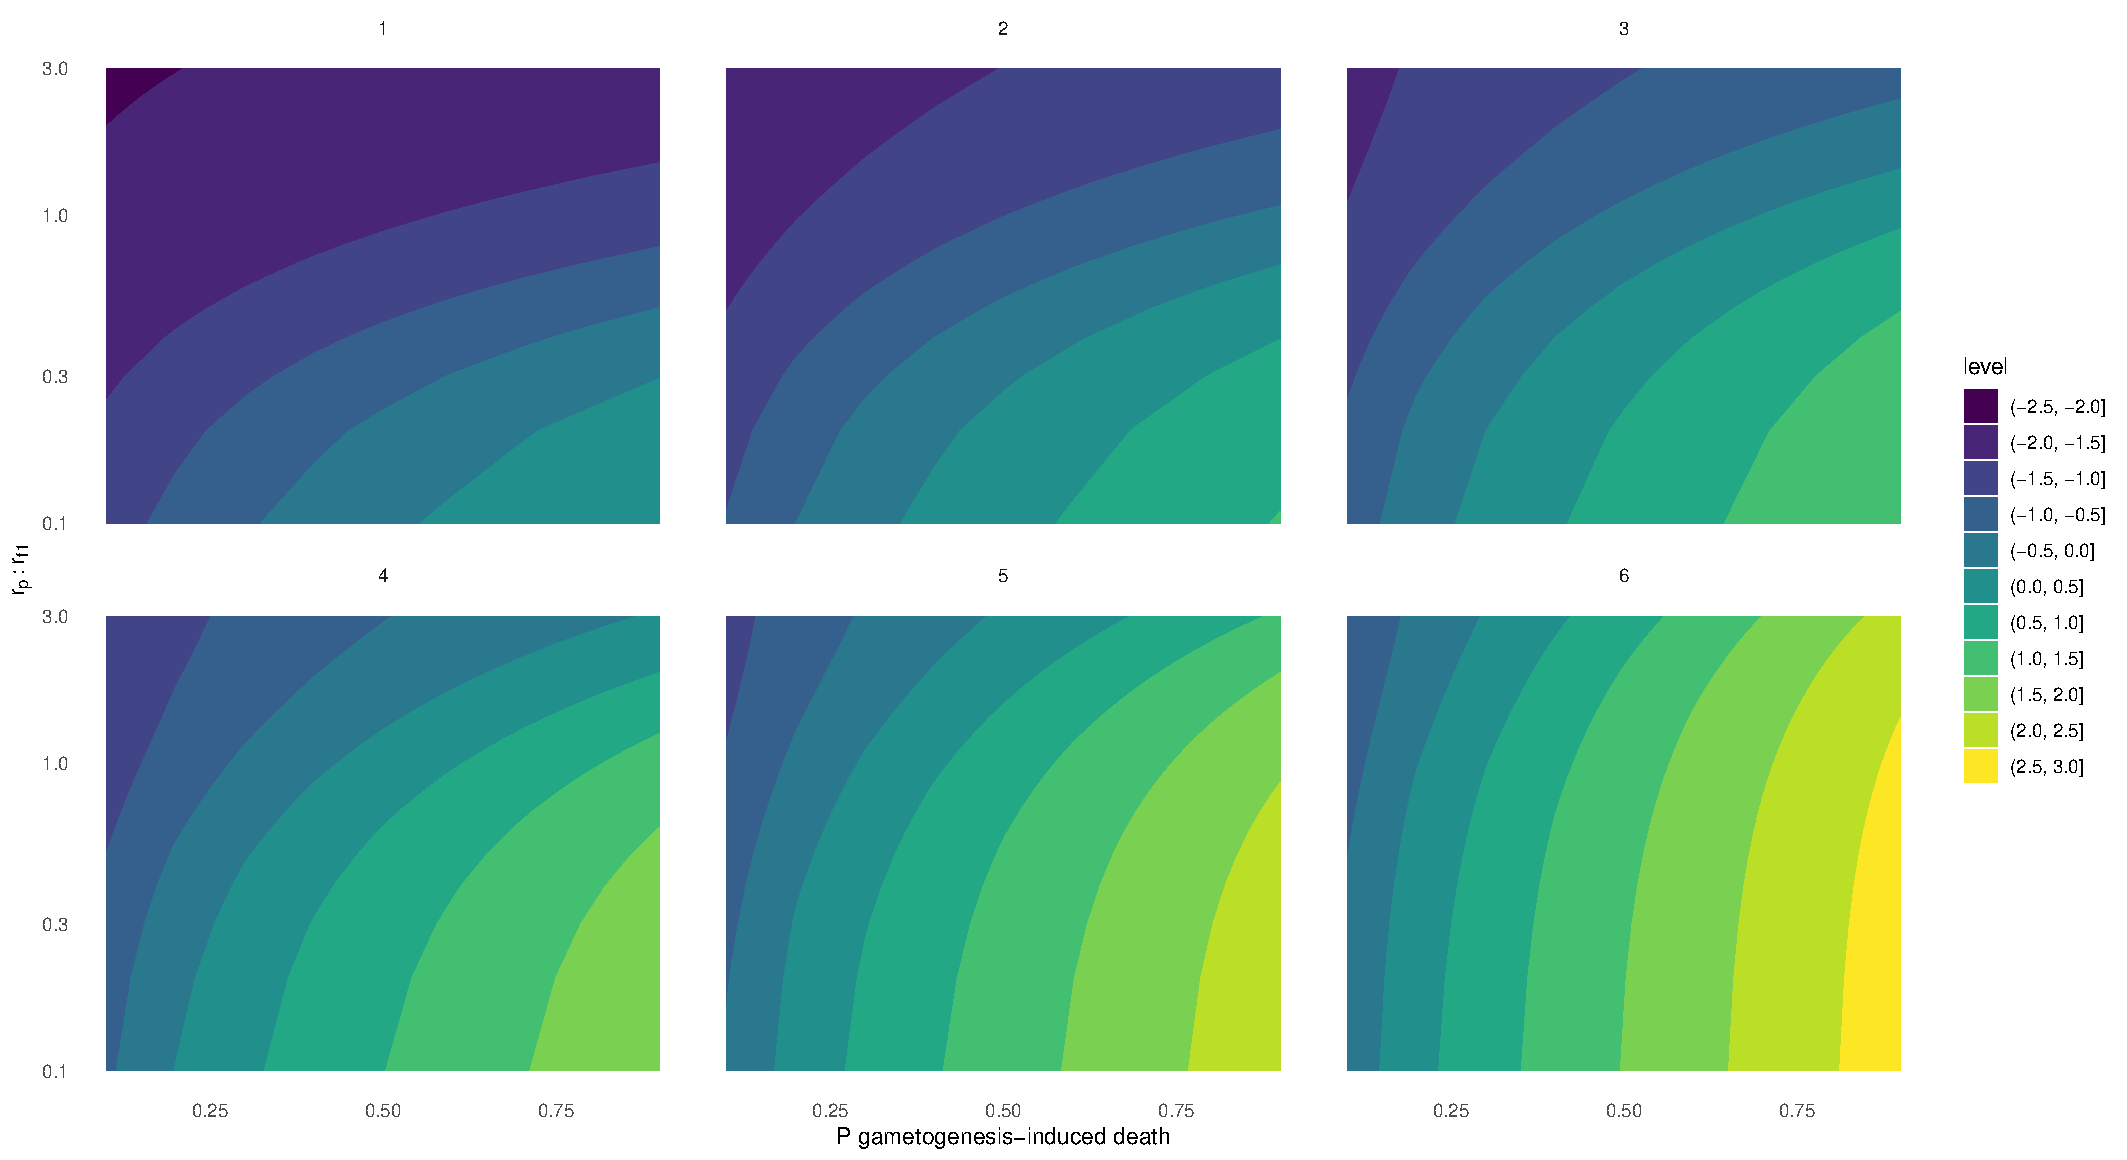
\includegraphics[width=\linewidth]{imgs/a.pdf}
      \end{subfigure}

      \begin{subfigure}{\textwidth}
        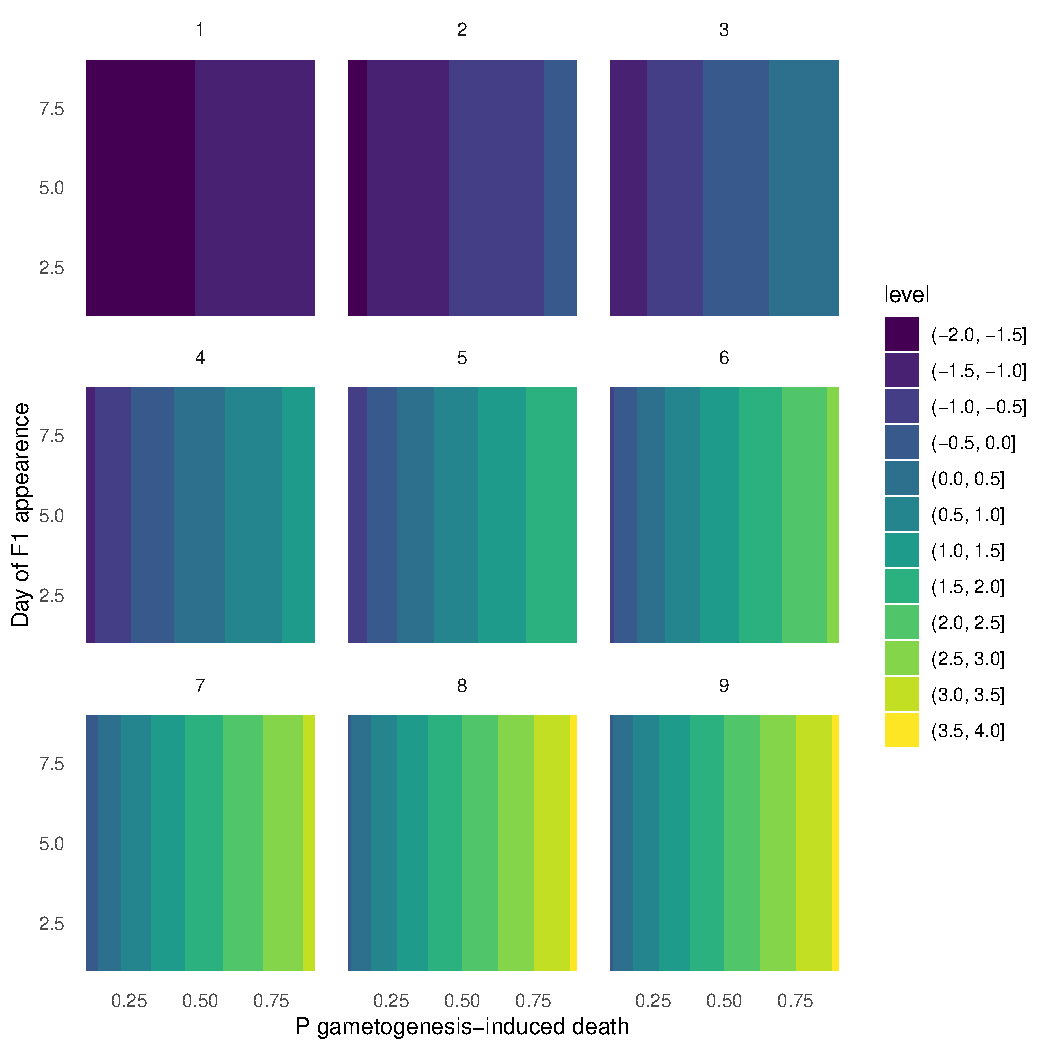
\includegraphics[width=\linewidth]{imgs/b.pdf}
      \end{subfigure}
      \caption{\textbf{Contour plots of ranges of recruitment success after 10 days of simulation for paired values of parameters (axes labels).}
        Recruitment success is expressed as $\log_{10}(F_{1}/P)$; $\alpha$ is the fraction of $P$ cells that will generate $F_{1}$.
        Different subplots represent different durations of growth arrest ($t_{AE}$ model parameter).
        Parameters left unchanged during the simulations were assigned as per \textbf{Tab.~\ref{tbl1}}.
      }\label{swep}
    \end{figure}
    %
    \begin{table}[p]
      \centering
      {%
        \begin{subtable}{12cm}\centering\scriptsize
          {
\begin{tabular}{lrrrrrrrrr}
\toprule
  & 0.01 & 0.03 & 0.05 & 0.08 & 0.1 & 0.12 & 0.15 & 0.17 & 0.2\\
\midrule
3 & -1.72 & -1.23 & -1.00 & -0.79 & -0.68 & -0.59 & -0.48 & -0.42 & -0.34\\
2.7 & -1.71 & -1.23 & -1.00 & -0.78 & -0.68 & -0.59 & -0.48 & -0.42 & -0.34\\
2.5 & -1.71 & -1.23 & -1.00 & -0.78 & -0.68 & -0.59 & -0.48 & -0.42 & -0.34\\
2.2 & -1.71 & -1.22 & -0.99 & -0.78 & -0.67 & -0.59 & -0.48 & -0.42 & -0.33\\
2 & -1.70 & -1.22 & -0.99 & -0.77 & -0.67 & -0.58 & -0.47 & -0.41 & -0.33\\
\addlinespace
1.7 & -1.70 & -1.21 & -0.98 & -0.77 & -0.66 & -0.58 & -0.47 & -0.41 & -0.33\\
1.5 & -1.69 & -1.20 & -0.98 & -0.76 & -0.66 & -0.57 & -0.47 & -0.41 & -0.33\\
1.2 & -1.67 & -1.19 & -0.96 & -0.75 & -0.65 & -0.56 & -0.46 & -0.40 & -0.32\\
1 & -1.66 & -1.18 & -0.95 & -0.74 & -0.63 & -0.55 & -0.45 & -0.39 & -0.31\\
\bottomrule
\end{tabular}
}
          \caption{$\alpha, r_p:r_{f1}, \text{with } d = 0.2$}
        \end{subtable}
        \\
       \vspace{0.5cm}
        \begin{subtable}{12cm}\centering\scriptsize
          {
\begin{tabular}{lrrrrrrrrr}
\toprule
  & 0.01 & 0.03 & 0.05 & 0.08 & 0.1 & 0.12 & 0.15 & 0.17 & 0.2\\
\midrule
3 & -1.69 & -1.20 & -0.96 & -0.74 & -0.63 & -0.53 & -0.41 & -0.34 & -0.24\\
2.7 & -1.68 & -1.19 & -0.96 & -0.73 & -0.62 & -0.52 & -0.40 & -0.33 & -0.24\\
2.5 & -1.68 & -1.19 & -0.95 & -0.72 & -0.61 & -0.52 & -0.40 & -0.33 & -0.23\\
2.2 & -1.67 & -1.18 & -0.94 & -0.71 & -0.60 & -0.50 & -0.38 & -0.31 & -0.22\\
2 & -1.66 & -1.17 & -0.93 & -0.70 & -0.59 & -0.49 & -0.37 & -0.30 & -0.21\\
\addlinespace
1.7 & -1.64 & -1.15 & -0.91 & -0.68 & -0.57 & -0.47 & -0.35 & -0.28 & -0.19\\
1.5 & -1.62 & -1.13 & -0.89 & -0.67 & -0.55 & -0.46 & -0.33 & -0.26 & -0.17\\
1.2 & -1.59 & -1.09 & -0.86 & -0.63 & -0.51 & -0.42 & -0.29 & -0.22 & -0.13\\
1 & -1.55 & -1.05 & -0.81 & -0.58 & -0.47 & -0.37 & -0.25 & -0.18 & -0.09\\
\bottomrule
\end{tabular}
}
          \caption{$\alpha, r_p:r_{f1}, \text{with } d = 0.4$}
        \end{subtable}
        \\
       \vspace{0.5cm}
        \begin{subtable}{12cm}\centering\scriptsize
          {
\begin{tabular}{lrrrrrrrrr}
\toprule
  & 0.01 & 0.03 & 0.05 & 0.08 & 0.1 & 0.12 & 0.15 & 0.17 & 0.2\\
\midrule
3 & -0.92 & -0.42 & -0.18 & 0.05 & 0.16 & 0.25 & 0.36 & 0.41 & 0.49\\
2.7 & -0.87 & -0.37 & -0.13 & 0.10 & 0.20 & 0.29 & 0.40 & 0.45 & 0.53\\
2.5 & -0.84 & -0.34 & -0.09 & 0.13 & 0.24 & 0.32 & 0.43 & 0.48 & 0.55\\
2.2 & -0.78 & -0.27 & -0.03 & 0.19 & 0.30 & 0.38 & 0.48 & 0.53 & 0.60\\
2 & -0.72 & -0.22 & 0.02 & 0.24 & 0.34 & 0.42 & 0.52 & 0.57 & 0.63\\
\addlinespace
1.7 & -0.62 & -0.12 & 0.11 & 0.32 & 0.42 & 0.49 & 0.58 & 0.63 & 0.68\\
1.5 & -0.54 & -0.04 & 0.19 & 0.39 & 0.48 & 0.55 & 0.63 & 0.67 & 0.72\\
1.2 & -0.36 & 0.11 & 0.32 & 0.50 & 0.58 & 0.64 & 0.71 & 0.74 & 0.79\\
1 & -0.20 & 0.24 & 0.43 & 0.58 & 0.65 & 0.70 & 0.76 & 0.79 & 0.83\\
\bottomrule
\end{tabular}
}
          \caption{$\alpha, r_p:r_{f1}, \text{with } d = 0.6$}
        \end{subtable}
        \caption{Tabular data of $\log_{10}(F_{1}/P)$ for different values of parameters showed at bottom and growth arrest duration of four days. All other parameters were assigned as per \textbf{Tab.~\ref{tbl1}}}\label{tbl2}
      }
    \end{table}
%
  \section*{Assumptions} 
    \begin{enumerate}
      \item I assume that net growth rate is the difference between size-dependent cell growth and death
      \item I assume that $P$ suffers extra mortality during growth arrest due to gametogenesis
      \item I assume that lenght decreases 0.1 um after each division
      \item I assume that $P$ has reached the environmental carrying capacity before starting the simulation
    \end{enumerate}
\end{document}
